%  ========================================================================
%  David P. Fleming's Thesis - University of Washington, Department of Astronomy, 2020
%  ========================================================================

%  ========================================================================
%  Copyright (c) 1985 The University of Washington
%
%  Licensed under the Apache License, Version 2.0 (the "License");
%  you may not use this file except in compliance with the License.
%  You may obtain a copy of the License at
%
%      http://www.apache.org/licenses/LICENSE-2.0
%
%  Unless required by applicable law or agreed to in writing, software
%  distributed under the License is distributed on an "AS IS" BASIS,
%  WITHOUT WARRANTIES OR CONDITIONS OF ANY KIND, either express or implied.
%  See the License for the specific language governing permissions and
%  limitations under the License.
%  ========================================================================
%

% Documentation for University of Washington thesis LaTeX document class
% by Jim Fox
% fox@washington.edu
%
%    Revised for version 2015/03/03 of uwthesis.cls
%    Revised, 2016/11/22, for cleanup of sample copyright and title pages
%
%    This document is contained in a single file ONLY because
%    I wanted to be able to distribute it easily.  A real thesis ought
%    to be contained on many files (e.g., one for each chapter, at least).
%
%    To help you identify the files and sections in this large file
%    I use the string '==========' to identify new files.
%
%    To help you ignore the unusual things I do with this sample document
%    I try to use the notation
%       
%    % --- sample stuff only -----
%    special stuff for my document, but you don't need it in your thesis
%    % --- end-of-sample-stuff ---


%    Printed in twoside style now that that's allowed
%
 
\documentclass [11pt, proquest]{uwthesis}[2016/11/22] % draft

\usepackage{amsmath,amssymb}
\usepackage{aasmacros}
\usepackage[version=4]{mhchem}
\usepackage{comment}
\usepackage{multirow,tabularx}
\usepackage{deluxetable}
\usepackage{mathtools,upgreek}
\usepackage{floatrow}
\usepackage{outlines}
\usepackage{setspace}
\usepackage{caption}
\usepackage{sidecap}
\captionsetup[table]{font={stretch=1.0}}     %% change 1.2 as you like
\captionsetup[figure]{font={stretch=1.0}}    %% change 1.2 as you like
\usepackage{epigraph}
\usepackage{times}
\usepackage{mathptmx}
\usepackage{bibentry}
\usepackage{xspace}
\usepackage{graphicx}
\usepackage[ruled,vlined]{algorithm2e}
\usepackage[round]{natbib}
\usepackage{xcolor}
\usepackage{import}

\PassOptionsToPackage{hyphens}{url}
 \usepackage[
     pdfauthor={David Paul Fleming},
    pdftitle={Inferring the Evolutionary Histories of Stars and Their Planets},
    pdfsubject={Astronomy},
    pdfcreator={pdflatex},
    bookmarks=true,         % show bookmarks bar?
     pdfnewwindow=true,      % links in new window
     colorlinks=true,    % false: boxed links; true: colored links
     linkcolor=xlinkcolor,     % color of internal links
     citecolor=xlinkcolor,     % color of links to bibliography
     filecolor=xlinkcolor,  % color of file links
     urlcolor=xlinkcolor,      % color of external links
     pdfpagemode=UseOutlines,
    final=true
    ]{hyperref}
\usepackage{hypcap}

%% Custom commands
\def\mearth{{\rm\,M_\oplus}}
\def\rearth{{\rm\,R_\oplus}}
\def\msun{{\rm\,M_\odot}}
\def\rsun{{\rm\,R_\odot}}
\def\lsun{{\rm\,L_\odot}}
\def\gsim{~\rlap{$>$}{\lower 1.0ex\hbox{$\sim$}}}
\def\lsim{~\rlap{$<$}{\lower 1.0ex\hbox{$\sim$}}}
\newcommand{\xxx}[1]{{\textbf{#1}}}
\newcommand{\vplanet}[0]{\texttt{VPLanet}\xspace}
\newcommand{\emcee}[0]{\texttt{emcee}\xspace}
\newcommand{\approxposterior}[0]{\texttt{approxposterior}\xspace}
\newcommand{\eqtide}[0]{\texttt{EQTIDE}\xspace}
\newcommand{\stellar}[0]{\texttt{STELLAR}\xspace}
\newcommand{\kepler}[0]{\textit{Kepler}\xspace}
\newcommand{\tess}[0]{\texttt{TESS}\xspace}
\newcommand{\jwst}[0]{\textit{JWST}\xspace}
\newcommand{\binary}[0]{\texttt{BINARY}\xspace}
\newcommand{\rebound}[0]{\texttt{REBOUND}\xspace}
\newcommand{\um}{$\upmu$m}

%% for editing changes
% hyperref link defaults to "blue" (0000ff) as this matches our publisher produced pdf style
\definecolor{xlinkcolor}{cmyk}{0.5,0.5,0,1}

\def\bibpreamble{\protect\addcontentsline{toc}{chapter}{Bibliography}}

\setcounter{tocdepth}{2}  % Print the chapter and sections to the toc
 

% ==========   Local defs and mods
%

\begin{document}
 
% ==========   Preliminary pages
%
% ( revised 2012 for electronic submission )
%

\prelimpages
 
%
% ----- copyright and title pages
%
\Title{Inferring the Evolutionary Histories of Stars and Their Planets}
\Author{David Paul Fleming}
\Year{2020}
\Program{Astronomy}

\Chair{Rory Barnes}{Professor}{Astronomy}
\Signature{Tom Quinn}
\Signature{Victoria Meadows}
\Signature{Jacob VanderPlas}
\Signature{Michael Johnson (GSR)}

% may be first or second. Must follow specified order. 
\titlepage  

\newpage

% May be first or second.
\copyrightpage

%
% ----- signature and quoteslip are gone
%

%
% ----- abstract
%

\begin{comment}
The abstract should use a paragraph to summarize each chapter:

\end{comment}



\setcounter{page}{-1}
\abstract{%

Abstract text. 

}


%
% ----- contents & etc.
%

\tableofcontents
\listoffigures
\listoftables  % I have no tables
 
%
% ----- glossary 
%
%\chapter*{Glossary}      % starred form omits the `chapter x'
\addcontentsline{toc}{chapter}{Glossary}
\thispagestyle{plain}
%
\begin{glossary}
\item[argument] replacement text which customizes a \LaTeX\ macro for
each particular usage.
\item[back-up] a copy of a file to be used when catastrophe strikes
the original.  People who make no back-ups deserve
no sympathy.
\item[control sequence] the normal form of a command to \LaTeX.
\item[delimiter] something, often a character, that indicates
the beginning and ending of an argument.
More generally, a delimiter is a field separator.
\item[document class] a file of macros that tailors \LaTeX\ for
a particular document.  The macros described by this thesis
constitute a document class.
\item[document option] a macro or file of macros
that further modifies \LaTeX\ for
a particular document.  The option {\tt[chapternotes]}
constitutes a document option.
\item[figure] illustrated material, including graphs,
diagrams, drawings and photographs.
\item[font] a character set (the alphabet plus digits
and special symbols) of a particular size and style.  A couple of fonts
used in this thesis are twelve point roman and {\sl twelve point roman
slanted}.
\item[footnote] a note placed at the bottom of a page, end of a chapter,
or end of a thesis that comments on or cites a reference
for a designated part of the text.
\item[formatter] (as opposed to a word-processor) arranges printed
material according to instructions embedded in the text.
A word-processor, on the other hand, is normally controlled
by keyboard strokes that move text about on a display.
\item[\LaTeX] simply the ultimate in computerized typesetting.
\item[macro]  a complex control sequence composed of 
other control sequences.
\item[pica] an archaic unit of length.  One pica is twelve points and
six picas is about an inch.
\item[point] a unit of length.  72.27 points equals one inch.
\item[roman]  a conventional printing typestyle using serifs.
the decorations on the ends of letter strokes.
This thesis is set in roman type.
\item[rule] a straight printed line; e.g., \hrulefill.
\item[serif] the decoration at the ends of letter strokes.
\item[table] information placed in a columnar arrangement.
\item[thesis] either a master's thesis or a doctoral dissertation.
This document also refers to itself as a thesis, although it
really is not one.
 
\end{glossary}
 

%
% ----- acknowledgments
%
\acknowledgments{% \vskip2pc
  % {\narrower\noindent
Acknowledgement statement.
  % \par}
}
%
% ----- dedication
%
\dedication{\begin{center}To my wife, Anya\end{center}}

%
% end of the preliminary pages
 
%
% ==========      Text pages
%

\textpages
 
% ========== Chapters

% intro
\chapter{Introduction}

\section{Some Models Are Useful}

Planets are inextricably linked to their host stars through their common birth environment. The fate of binary stars is similarly intertwined.  As such, numerous coupled astrophysical processes ranging from tidal forces \citep{Zahn1989,Barnes2017} to stellar high-energy emission \citep{Airapetian2019} shape the long-term evolution of both stellar and planetary systems. Modern astronomical surveys have produced a wealth of information to help elucidate the processes that dictate this evolution. Notably, completed surveys such as \kepler \citep{Borucki2003,Borucki2010}, \textit{K2} \citep{Howell2014}, and the in-progress Transiting Exoplanet Survey Satellite \citep[\textit{TESS}, ][]{Ricker2014} have monitored the brightness variation of well over 100,000 stars to detect transiting exoplanets and eclipsing binary stars, massively increasing the known population of such systems.  These large amounts of data and the promise of future missions, e.g. the \textit{James Webb Space Telescope} (\textit{JWST}), present an unprecedented opportunity for both population-level statistical studies and individual target characterization to infer the fundamental properties and processes that govern the evolution stars and their planets.

An unavoidable problem for these efforts within the discipline of astronomy, however, is that the timescales over which astrophysical processes operate are often much, much longer than the lifetime of a single astronomer, or even the duration of recorded human history. For example, the main sequence lifetime of Sun-like stars is of order 10 Gyrs \citep{Baraffe2015}, a factor of $10^7$ longer than an optimistic estimate for the lifetime of a person. How can astronomers hope to learn about the long-term evolution of such objects if they can only observe brief snapshots of the cosmos over time? The fundamental problems of astronomy are therefore given what is observed, how can astronomers infer what physical processes produced the observations and what does this information imply about the past and future evolution? 

Theoretical models are critical for the interpretation of observed data and are required to understand the past and future evolution of astrophysical objects. These models provide mathematical descriptions of the underlying physical processes that permit researchers to examine how said processes operate. Researchers can then confront model predictions with data to assess their validity and characterize the underlying processes at play. For example, consider the classic problem in astronomy of understanding how and why the planets trace their apparent orbits in the night sky. In his famous work colloquially referred to as the \textit{Principia}, Newton developed the well-known inverse square law model for gravity. In his model, Newton postulated that the gravitational force that attracts massive bodies together depends on the square of their separation and the product of their masses \citep{Newton1687,Newton1999}. Newton demonstrated how his model naturally reproduces the observed elliptical orbits of the planets in the Solar System and hence offers a reasonable explanation for the underlying physics. Moreover, this model has been used to study a vast array of astrophysical phenomena including the orbits of exoplanets and galactic dynamics. Successful theoretical models offer both an explanation for the underlying processes and are able to predict the physical consequences of these mechanisms.

Theoretical models are inherently imperfect, however, as one typically must make simplifying assumptions to make evaluating the model tractable, but mostly because one often does not have a full understanding of the processes that govern the evolution of the system in question. The Newtonian theory of gravity was wildly successful\footnote{I use the inverse square law for gravity, and theories derived from it, e.g. equilibrium tides \citep{Darwin1880}, extensively in this dissertation, for example.}, but ultimately limited as it failed to explain the perihelion precession of Mercury, for example. These general issues for models are simply summarized by the well-known aphorism
\begin{quote}
All models are wrong. - \citet{Box1976}
\end{quote}
As I build theoretical models in this dissertation, I will often revisit the spirit of this quote to identify the limitations of my models and how they could be improved in future work.

Astronomers' understanding of the Universe is always advancing. Much later after Newton, Einstein identified the need for a more mathematically-complex theory to better explain the force of gravity and its consequences. In his theory of ``General Relativity," Einstein showed how a nonlinear tensor field description of gravity provides a compelling explanation for numerous unexplained gravitational phenomena, including the perihelion precession of Mercury \citep{Einstein1915b,Einstein1915a}. Thus as science proceeds and observations are made, theoretical models must be derived and continually improved to interpret and explain what we see in the world around us. In this dissertation, I make much more humble theoretical contributions than the previously noted authors to understand the evolution of stars and their planets. 

\section{Much Ado About Data}

The parameters of theoretical models represent physically meaningful quantities, like a star's mass, that we hope to constrain with data and use to understand the underlying astrophysical processes at work. With data, one can apply a model to infer parameters. For example in this dissertation, I apply my model for coupled stellar-tidal evolution to measurements of the orbital and rotational properties of \kepler eclipsing binaries \citep[e.g.][]{McQuillan2014,Lurie2017}. With my model, I can simulate the dynamics of such systems to constrain model parameters and understand their long-term evolution. But what about the case where astronomers have yet to observe the object or phenomenon in question?

In situations where observations have not yet been made, e.g. the detection of a terrestrial exoplanetary atmosphere, theoretical models can be used to make useful predictions.  When future facilities like \textit{JWST} attempt to characterize terrestrial exoplanetary atmospheres in the search for biosignatures, for example, astronomers will use complex radiative transfer codes to estimate atmospheric compositions \citep[e.g. SMART,][]{Meadows1996,Crisp1997}. Critical to understanding and interpreting these results is determining how the exoplanet and its atmosphere evolved to its present state. This evolution necessarily depends on the long-term evolution of the planet's host star because the stellar high-energy XUV luminosity (X-ray and extreme ultraviolet emission ranging over approximately 1-1000\AA) drives volatile escape processes that have been shown to dramatically impact exoplanetary atmospheres \citep{Watson1981,Lammer2003,MurrayClay2009}. For example, \citet{Luger2015} showed via theory and simulation how the large pre-main sequence luminosities of low-mass stars can drive water photolysis and hydrogen loss from terrestrial exoplanets during an extended runaway greenhouse phase. This photolysis can cause extreme amounts of O$_2$ to build up in the planets' atmospheres, up to 1000s of bars, significantly impacting absorption features in their spectra and the prospects for identifying true positive biosignatures \citep[see][]{Meadows2017,Meadows2018}. Modeling the long-term evolution of astrophysical systems that consider the relevant physics is critical to the estimation of their present state. Later in this dissertation, I further examine this problem by constructing a model for the long-term XUV evolution of TRAPPIST-1. I consider its impact on TRAPPIST-1's planetary system because \textit{JWST} will likely focus its search for life-bearing exoplanets on the TRAPPIST-1 planetary system \citep{Morley2017,Lincowski2018,Lustig2019}. 

When data are available, astronomers can infer information about astrophysical systems and the processes that govern them using models. Model predictions can then be conditioned on the observations to derive constraints on parameters. Many theoretical studies that examine the long-term evolution of systems to interpret observations and constrain parameters do so in the form of ``best fit models" by finding the set of model parameters that most closely reproduce the observations, within the uncertainties.  This technique is useful and informative, but ultimately insufficient, however, as a robust analysis used to interpret observations must be based in a probabilistic framework in which model predictions are conditioned on the data. Moreover, any constrained parameter requires an uncertainty estimation to permit a credible interpretation of the results.  For example if a forward model yields a best fit prediction of 1 Earth ocean of liquid surface water remaining on an Earth-sized exoplanet, one might infer that this exoplanet could be habitable like Earth. However, how credible is this interpretation?  If instead in this example one propagated data uncertainties through the forward model to find that the remaining surface water content is 1$^{+10}_{-1}$ Earth oceans, the planet's current state ranges from desiccated to water-rich, with both cases entirely consistent with the observations, yet indicative of significantly different evolutionary histories. Similar analogies can be made for any quantity an astronomer would like to measure, e.g. stellar masses, ages, binary orbital eccentricities, etc.

To address this issue, one can use theoretical models to constrain unobserved processes while robustly accounting for data uncertainties using the statistical method of Bayesian inference. Generally, Bayesian inference proceeds as follows:  One seeks to derive a probability distribution for model parameters, e.g. a star's mass given its observed luminosity and a model for stellar evolution.  That distribution should quantify how likely it is that the parameter takes on certain values and capture the inherent uncertainty in the parameter values given data.  This distribution is known as the ``posterior probability distribution" and accounts for observed data, the data uncertainties, parameter correlations, and one's prior belief about how the parameters are distributed. To compute the posterior distribution of model parameters, \textbf{x}, given observed data, $Data$, one applies Bayes' Theorem: 
\begin{equation} \label{intro:eqn:bayes}
P(\textbf{x} | Data) \propto P(Data | \textbf{x}) P(\textbf{x}),
\end{equation}
where $P(\textbf{x} | Data)$ is the posterior probability of \textbf{x} given $Data$, $P(\textbf{x})$ is the prior probability assigned to \textbf{x}, and $P(Data | \textbf{x})$ is the probability of the $Data$ given \textbf{x}, commonly referred to as the ``likelihood" of $Data$ given \textbf{x}. This equation neglects the normalization constant, $1/P(Data)$, as this is typically quite difficult to compute in practice because it requires integrating the likelihood over the prior. Through Bayes' Theorem, the posterior probability can be thought of as using data to update one's prior belief of how $\textbf{x}$ is distributed, given a model for the likelihood of the data. Note that in this dissertation, I will use the natural logarithm of Bayes' Theorem and refer to $\ln P(\textbf{x} | Data)$ to as the ``lnprobability". For notational convenience, I define the lnprobability as $f(\textbf{x})$. See Chapters 5 and 6 for additional discussion and a practical application of this definition. 

\section{More Ado about CPU Cycles}

In this dissertation, I built theoretical models for the long-term evolution of single and binary stars and considered what impact this evolution had on the stars' planets given available data. I implemented these models in \vplanet\footnote{VPLanet is publicly available
at \href{https://github.com/VirtualPlanetaryLaboratory/vplanet}{{https://github.com/VirtualPlanetaryLaboratory/vplanet}}.}, a modular, open-source code written in C that simulates the evolution of stellar and exoplanetary systems subject to a wide range of coupled astrophysical processes \citep{Barnes2019}. When performing Bayesian inference with \vplanet, I must compute the likelihood by running a simulation to make a prediction, e.g. a stellar binary's orbital period after Gyrs of tidal evolution, and compare it to the observed value and associated uncertainty. This comparison is typically performed using a $\chi^2$ statistic if the uncertainties are assumed to be Gaussian and uncorrelated, a standard assumption. 

Since this inference requires running a \vplanet simulation, the posterior distribution is not an analytic function. Moreover, I cannot reasonably compute the normalization term in Bayes' Theorem, $1/P(Data)$, so I must use a Monte Carlo sampling technique to estimate the posterior distribution. This procedure is usually performed using Markov chain Monte Carlo (MCMC) methods such as the affine-invariant MCMC code, \emcee, whose usage is seemingly ubiquitous in modern astronomy \citep{ForemanMackey2013}. MCMC methods are incredibly powerful as they simply require computing a function that is proportional to the posterior probability, e.g. the likelihood times the prior for a given \textbf{x}, allowing them to neglect the normalization term and directly sample from the posterior distribution. How the sampling proceeds depends on the MCMC algorithm, but generally given long enough MCMC chains, the derived distributions are asymptotically guaranteed to converge to the correct distribution, ensuring credible results when using an appropriate theoretical model. Standard MCMC runs often require at least $10^6$ likelihood calculations to draw a suitable number of samples from the posterior distribution and build up statistical power, however. Depending on the dimensionality of the problem, i.e. how many model parameters one wishes to constrain, MCMC chains can require drawing many more samples.

Consider the coupled stellar-tidal dynamical evolution of binary stars, a case examined throughout this dissertation. Due to a combination of stellar evolution and tidal gravitational forces, stellar spins and the binary orbit evolve over long timescales, dramatically impacting their observed properties and the evolution of any planetary systems they might host \citep[for example, see][for how tides circularize binary orbits over time]{Zahn1989,Meibom2005}. A reasonable model of this evolution must at least account for stellar evolution \citep[e.g.][]{Baraffe2015}, tidal evolution \citep[e.g.][]{Hut1981,FerrazMello2008,Leconte2010}, and stellar magnetic braking \citep[e.g.][]{Matt2015}. Simulating this evolution with \vplanet would therefore require setting many initial conditions for each of the modules that control these physical effects, e.g. the stellar masses, initial orbital eccentricity, initial stellar spins, etc.  As the number of input parameters, and hence simulation dimensionality, increases, systematically exploring parameter space with simulations to understand model predictions and the underlying physics becomes infeasible as the number of required simulations grows exponentially with dimensionality, the so-called ``Curse of Dimensionality" \citep{Bellman1957}.  Not only is Bayesian inference with numerical models often slow due to the requisite number of MCMC samples, it is significantly hampered by the ``Curse of Dimensionality". Given these significant computational issues, Bayesian inference with complicated models that account for the relevant physical processes, e.g. Bayesian inference with \vplanet, often becomes computationally-intractable.

In this dissertation, I explored how the growing field of machine learning can solve these problems. Machine learning is a powerful application of computer science and statistics in which a predictive algorithm ``learns" complex patterns in data to make predictions on unseen data \citep[see][for a thorough review]{Murphy2012}. The key step in using a supervised machine learning algorithm is training, i.e. calibrating the predictive model based on a subset of known outcomes.  A probabilistic predictive machine learning model trained on the results of \vplanet simulations, for example, could predict the end result of stellar-tidal evolution in binary stars, with an associated uncertainty, without actually performing the simulations.  Within the field of astronomy in the past few years, the application of supervised machine learning has become rather common. For example, \citet{Lam2018} applied supervised machine learning to successfully predict the results of complex simulations of circumbinary planet stability whereas \citet{Waldmann2016} used machine learning to predict exoplanet atmospheric chemical abundances given transmission spectra. Clearly, machine learning provides promising new methods that help predict the results of simulations and infer model parameters given data. With a trained machine learning model, I could replace running computationally expensive simulations to enable Bayesian inference with my models, solving this issue. 

In this dissertation, I developed theoretical models to probe and infer the long-term evolution of single and binary stars given data. My research focused on the dynamical evolution of such systems and how it impacts their surrounding planetary systems. I extended my theoretical modeling to infer the evolving high-energy radiation environment experienced by the TRAPPIST-1 planetary system by comparing my models with observations of TRAPPIST-1 using Bayesian statistics. I developed and applied a novel machine learning software package to this inference problem and demonstrated its promise for enabling Bayesian inference with computationally expensive models. Below, I provide an outline for this dissertation and briefly highlight my results. 

\section{Dissertation Outline}

In Chapter 2, I study the dynamics of the birth environment of circumbinary exoplanets by running an ensemble of smooth particle hydrodynamic (SPH) N-body simulations of circumbinary protoplanetary disks. My work demonstrates that these dynamically-rich disks coevolve with their central host binary stars by exchanging angular momentum through gravitational resonances, ultimately driving the orbital evolution of both the binary and the inner-edge of the disk where planets can form and migrate. In Chapter 3, I extend my work with circumbinary planetary systems and develop a model to explain the observed lack of circumbinary planets (CBPs) orbiting short-period binary stars in the \kepler field. By constructing a theoretical model for the coupled stellar-tidal evolution of binary stars, I show that the expanding orbits of young binaries can efficiently destabilize CBPs that orbit just exterior to the dynamical stability limit, explaining their observed dearth.

I continue my work with binary stars in Chapter 4 to explore how the competition between tidal torques and magnetic braking in binaries can shape the observed rotation period distribution of low-mass main sequence stars in the \kepler field. I show how my model reproduces previously-unexplained stellar populations in the \kepler field such as the subsynchronous eclipsing binary stars identified by \citet{Lurie2017}. I apply my theory to identify major limitations of the stellar age determination method of gyrochronology when it is erroneously applied to unresolved stellar binaries. I then explore how my model's predictions could be used in tandem with future observations to distinguish between which equilibrium tidal theory best describes tidal interactions in main sequence low-mass binary stars.

In Chapter 5, I introduce \approxposterior, my open-source machine learning Python package for approximate Bayesian inference with computationally expensive models. I discuss the algorithm, its convergence properties, and provide example use cases. I then discuss how this efficient machine learning method can enable Bayesian inference studies for a wide array of computationally expensive inference problems. In Chapter 6, I combine theory, Bayesian inference, and machine learning to infer the long-term high-energy radiation environment experienced by the TRAPPIST-1 planetary system, the current best target for the detection and characterization of terrestrial planet atmospheres by \textit{JWST}. I construct a probabilistic model for TRAPPIST-1's evolving XUV luminosity, conditioning the inference on both observations of TRAPPIST-1 and of late M dwarfs. From this inference, I find that TRAPPIST-1 likely underwent an extended epoch of enhanced XUV emission, potentially driving extreme volatile loss from its planets and impacting what \textit{JWST} might observe in future observations. I demonstrate that this Bayesian inference is too computationally expensive to scale to either a larger number of stars or inference with a more complex model. To address this concern, I apply \approxposterior to the TRAPPIST-1 inference problem. I demonstrate that it can accurately replicate the probabilistic analysis, but requires nearly three orders of magnitude fewer computational resources than \emcee.  Finally, I summarize my findings and discuss prospects for related future research.



% Models
\chapter{Resonant Dynamical Interactions Between Binary Stars and Circumbinary Disks}
%\include{tex/chapter1}

% XXX
\chapter{Coupled Stellar-Tidal Evolution Ejection of Circumbinary Exoplanets}
\import{tex/STEEP/}{bin_tides.tex}

\clearpage

% XXX
\chapter{Stellar Rotation Rates in Binary Stars: The Competition between Magnetic Braking and Tidal Torques}
\import{tex/sync/}{sync.tex}

% approxposterior
\chapter{Approximate Bayesian Inference with \approxposterior}
%\include{tex/chapter4}

% XXX
\chapter{Inferring the XUV History of the TRAPPIST-1 Planetary System}
%\include{tex/chapter4}

% Discussion
\chapter{Discussion}
%\section{Discussion}

This is where I discuss things.

\section{Conclusions}

Finally, I conclude.

% Conclusions
\chapter{Conclusions}
%In this dissertation, I developed theoretical and probabilistic models to understand and infer the long-term evolution of single and binary stars. Although my modeling efforts focus on the dynamical evolution of such systems, e.g. how and why a binary's orbit evolves over time, I considered what impact stellar and binary evolutionary processes have on planets orbiting the stars. I employed my models to examine different aspects of the lifetime of stellar and planetary systems, including early stellar interactions with a protoplanetary disk and the evolving high-energy radiation environment experienced by terrestrial planets orbiting late M-dwarfs throughout the pre-main sequence. I confronted my model predictions with observational data from NASA missions like \kepler to constrain unobserved model parameters and develop testable hypotheses for unexplained features in the data. Through my novel theories and inference methods, I explore how the past evolution of stars in planetary systems shape what we observe today.

Much of my work focused on developing a theoretical explanation for anomalous stellar and exoplanet populations discovered by \kepler. The recent discoveries of transiting circumbinary planets (CBPs) by \kepler, for example, raise questions for contemporary planet formation models \citep[see][]{Welsh2014}.  Understanding how these planets form requires characterizing their formation environment, the circumbinary protoplanetary disk, and how the disk and binary interact and change as a result.  In young circumbinary systems, the central binary excites gravitational resonances in the surrounding protoplanetary disk that drive evolution in both the binary orbit and in the disk, likely impacting forming and migrating planets.  In Chapter 2, I probed how these resonant interactions impact binary eccentricity and disk structure evolution by running an ensemble of N-body smooth particle hydrodynamics (SPH) simulations of gaseous protoplanetary disks surrounding binaries based on Kepler-38. I ran these large simulations for $10^4$ binary periods over several initial binary eccentricities, disk scale heights, and resolutions.  I demonstrated that nearly circular binaries weakly couple to the disk via a parametric instability and excite disk eccentricity growth, mostly near the inner-edge of the disk where planets form and migrate.  I showed that binaries with eccentric orbits strongly couple to the disk causing eccentricity growth for both the disk and binary orbit. Moreover, disks orbiting binaries with sufficient orbital eccentricity to strongly couple to the disk develop an $m = 1$ spiral wave launched from the 1:3 eccentric outer Lindblad resonance (EOLR) that corresponds to an alignment of gas particle longitude of periastrons. I found that all binaries also underwent semi-major axis decay due to dissipation from the viscous disk. I then considered how disk-binary interactions impacted the long-term binary dynamical evolution and the evolution and dynamical stability of any CBPs subject to this evolution. 

Curiously, \kepler has identified a distinct lack of transiting CBPs orbiting short period binary stars. One proposed explanation for this dearth is dynamical perturbations by a tertiary companion star coupled with tidal friction that shrinks the central binary and perturbs the CBP's orbit, possibly destabilizing it \citep{Munoz2015,Martin2015b,Hamers2016}.  However to date, no theory has been put forward to explain the lack of CBPs around isolated binaries, i.e. those without a tertiary. In Chapter 3, I posited a mechanism that explains the observed lack of CBPs via coupled stellar-tidal evolution of isolated binary stars. I demonstrated how tidal forces between low-mass, short-period binary stars on the pre-main sequence slow the stellar rotations, transferring rotational angular momentum to the orbit as the stars approach the tidally locked state.  This transfer increases the binary orbital period, expanding the region of dynamical instability around the binary, and ultimately destabilizing CBPs that tend to preferentially orbit just beyond the initial dynamical stability limit.  After the stars tidally lock, I found that angular momentum loss due to magnetic braking can significantly shrink the binary orbit, and hence the region of dynamical stability, over time impacting where surviving CBPs are observed relative to the boundary.  I performed simulations over a wide range of parameter space and found that the expansion of the instability region occurs for most plausible initial conditions and that in some cases, the stability semi-major axis doubles from its initial value.  I then examined the dynamical and observable consequences of a CBP falling within the dynamical instability limit by running N-body simulations of circumbinary planetary systems and found that typically at least one planet is ejected from the system.  I applied my theory to the shortest period \kepler binary that possesses a CBP, Kepler-47, and showed via simulation that its existence is consistent with my model.  Under conservative assumptions, I found that coupled stellar-tidal evolution of pre-main sequence binary stars removes at least one close-in CBP in $87\%$ of multi-planet circumbinary systems. I perform several sensitivity tests and found that my mechanism is effective for initial conditions that are generally consistent with observational and theoretical constraints of stellar and binary system orbital parameters. 

To discover transiting exoplanets, \kepler had to constantly observe the stars in its field, thereby creating a massive trove of the brightness modulations of many low-mass, main sequence stars over the course of the telescope's lifetime \citep{Borucki2003,Borucki2010}. By measuring these brightness variations as a function of time, astronomers can infer that some are caused by star spots moving in-and-out of the field of view, allowing astronomers to measure stellar rotation periods \citep[P$_{rot}$, see][]{McQuillan2014}. In Chapter 4, I extended my model for the long-term secular dynamical evolution of binary stars to examine how tides, stellar evolution, and magnetic braking shape the P$_{rot}$ evolution of low-mass stellar binaries in the \kepler field. I explored this evolution up to binary orbital periods (P$_{orb}$) of 100 d and across a wide range tidal dissipation parameters using two common equilibrium tidal models. I found that many binaries with P$_{orb} \lsim 20$ d tidally lock, and most with $P_{orb} \lsim 4$ d tidally lock into synchronous rotation on circularized orbits. At short P$_{orb}$, tidal torques produced a population of fast rotators that single-star only models of magnetic braking fail to produce.  I showed that in many cases, the competition between magnetic braking and tides produced a population of subsynchronous rotators that persisted for Gyrs, even in short P$_{orb}$ binaries, qualitatively reproducing the subsynchronous eclipsing binaries (EBs) discovered by \citet{Lurie2017} in the \kepler field. Both equilibrium tidal models predicted that binaries can tidally-interact out to P$_{orb} \approx 80$ d, while the Constant Phase Lag tidal model predicted that binaries can tidally lock out to P$_{orb} \approx 100$ d. Tidal torques often forced the P$_{rot}$ evolution of stellar binaries to depart from the long-term magnetic braking-driven spin down experienced by single stars, revealing that P$_{rot}$ is not be a valid proxy for age in all cases, i.e. gyrochronology can underpredict ages by up to $300\%$ unless one accounts for binarity. I concluded this Chapter by suggesting how accurate determinations of orbital eccentricties and P$_{rot}$ can be used to discriminate between which equilibrium tidal models best describes tidal interactions in low-mass binary stars.
 
In Chapter 5, I applied machine learning to enable Bayesian inference with computationally-expensive models. I introduced \approxposterior, an open source Python machine learning package for approximate Bayesian inference using Gaussian process (GP) regression. I implemented and generalized both the ``Bayesian Active Learning for Posterior Estimation" (BAPE, \citet{Kandasamy2017}) and ``Adaptive Gaussian process approximation for Bayesian inference with expensive likelihood functions" (AGP, \citet{Wang2018}) approximate Bayesian inference algorithms. For these algorithms, \approxposterior trains a GP to predict the posterior probability estimated by Bayes' Theorem for a set of model parameters by regressing on a small initial subset of forward model runs. The GP is used within an Markov Chain Monte Carlo (MCMC) sampling method, e.g. \emcee, to efficiently obtain an approximation to the posterior probability distribution, dramatically reducing the computational expense relative to obtaining the posterior using the computationally-expensive forward model. Moreover, I detailed how \approxposterior employs an active learning approach to iteratively improve the GP's predictive performance while minimizing the number of calls to the expensive model required to generate the GP's training set as an additional means of reducing the computational cost.  I outlined the steps that comprise \approxposterior's algorithm and explained how to assess convergence with practical examples and a Python script. I concluded by explaining how to use \approxposterior in conjunction with theoretical models as a general method for efficient approximate inference of unobserved model parameters given data.
 
In Chapter 6, I combined my theoretical modeling, machine learning, and Bayesian inference to model the long-term XUV luminosity evolution of TRAPPIST-1. TRAPPIST-1 is a prime target for atmospheric characterization with the James Webb Space Telescope \citep{Morley2017,Lincowski2018,Lustig2019}, and therefore constraining the evolving high-energy radiation environment experienced by its planetary system is critical to modeling their putative atmospheres and interpreting future observations. Using MCMC, I derived probabilistic constraints for TRAPPIST-1's stellar and XUV evolution that accounted for observational uncertainties, degeneracies between model parameters, and empirical data of low-mass stars. I constrained TRAPPIST-1's mass to $m_{\star} = 0.089 \pm{0.001}$ M$_{\odot}$ and found that its early XUV luminosity likely saturated at $\log_{10}(L_{XUV}/L_{bol}) = -3.03^{+0.23}_{-0.12}$. From the posterior distribution, I inferred that there is a ${\sim}40\%$ chance that TRAPPIST-1 is still in the saturated phase today, suggesting that TRAPPIST-1 has maintained high activity and $L_{XUV}/L_{bol} \approx 10^{-3}$ for several Gyrs. TRAPPIST-1's planetary system therefore likely experienced a persistent and extreme XUV flux environment, potentially driving significant atmospheric erosion and volatile loss. The inner planets likely received XUV fluxes ${\sim}10^3 - 10^4\times$ that of the modern Earth during TRAPPIST-1's ${\sim}1$ Gyr-long pre-main sequence phase. I showed how deriving these constraints via MCMC is computationally non-trivial, so scaling my methods to constrain the XUV evolution of a larger number of M dwarfs that harbor terrestrial exoplanets would incur significant computational expenses. I demonstrated that my open-source Python machine learning package, \approxposterior, accurately and efficiently replicates my analysis using 980 times less computational time and 1330 times fewer simulations than MCMC sampling using \emcee. I showed that \approxposterior derives constraints with mean errors on the best fit values and $1\sigma$ uncertainties of $0.61\%$ and $5.5\%$, respectively, relative to \emcee.

Developing a theory within a Bayesian framework allows modelers to appropriately account for data uncertainties and parameter correlations, an essential requirement for the estimation of the past evolution of stellar and planetary systems. Simulating the complex physical effects required to model this evolution while using Bayesian statistics will inevitably incur significant computational expenses, however, I have demonstrated that \approxposterior can enable such efforts. Future research can apply the methodology discussed above and presented in this thesis to provide insight into the histories of stars and their planets using the models implemented in \vplanet in conjunction with \approxposterior. By using a model with numerous physical effects, e.g. models for stellar evolution, water loss, and tidal dissipation, for example, I could build a probabilistic model for the long-term tidal and atmospheric evolution of some exoplanetary system to assess its present-day habitability and understand its past evolution given suitable observational constraints. 

This approach is of course not limited to the theoretical models implemented in \vplanet. For example, as I described in $\S$~\ref{AP:sec:future}, astronomers cannot directly observe the atmospheric chemical abundances that produce spectral absorption features in transmission spectroscopy observations. Instead, astronomers must infer these abundances from spectra using complex radiative transfer inverse modeling that matches model outputs to the data. In $\S$~\ref{AP:sec:future}, I presented results from an in-progress collaboration that demonstrated how \approxposterior can be used with the radiative transfer code SMART \citep{Meadows1996,Crisp1997} to perform atmospheric chemical abundance inference for a realistic model of an Earth-like TRAPPIST-1e (Lustig-Yaeger et al., in prep). Similar to the results discussed in Chapter 6, this inference requires nearly three orders of magnitude less computational resources than modern MCMC samplers like \emcee, demonstrating the promise of applying novel machine learning methods to Bayesian inference problems with computationally-expensive models.



% Appendix
%\chapter{Appendix: \approxposterior documentation}
%\textit{Portions of this chapter were originally published in collaboration with Jake VanderPlas in the September 2018 edition of the Journal of Open Source Software (\citet{FlemingVanderPlas2018}, JOSS, Vol. 3, 29, p. 781; 2018, DOI: 10.21105/joss.00781), and are reproduced below with permission of the Journal of Open Source Software. Portions of this chapter were originally published in collaboration with Rory Barnes, Rodrigo Luger, and Jacob VanderPlas in March 2020 in the Astrophysical Journal (\citet{Fleming2020}, ApJ, Vol. 891, 2; 2020 \textcopyright \ American Astronomical Society, DOI: 10.3847/1538-4357/ab77ad), and are reproduced below with permission of the American Astronomical Society.}

\

In this thesis, I have developed numerous theoretical models, all implemented in \vplanet, that simulate the long-term evolution of stars and their planets. In this Chapter, I consider how I can use those models to infer the evolutionary history of exoplanetary systems in conjunction with observational constraints using Bayesian statistics. I explain the significant numerical challenges that can make such studies intractable, motivating the development of a software package for rapid, approximate Bayesian inference, \approxposterior \citep{FlemingVanderPlas2018}. I describe the \approxposterior algorithm and implementation in detail, provide example use cases, and conclude by discussing in-progress and future work with \approxposterior. 

\section{Introduction}

As I discussed in the Introduction (Chapter 1), one can combine theoretical models, data, and Bayesian inference to constrain unobserved parameters. I am interested in applying the well-known statistical methodology of Bayesian inference with my theoretical models to infer the evolutionary history of stars and their planets (see Chapter 6). Consider, for example, an experiment in which I want to infer the stellar evolution of an M-dwarf and the long-term atmospheric escape experienced by its potentially-habitable exoplanet given some observed data, e.g. the star's age, the stellar and planetary masses, etc. \vplanet has reasonable physical models for both phenomena, so I could therefore use \vplanet within a Markov Chain Monte Carlo (MCMC) sampling algorithm to constrain the evolution. The MCMC yields the posterior probability distribution for model parameters that account for observational data, data uncertainties, and correlations between parameters, thereby permitting a robust inference of the process in question (assuming we have a suitable model).

For this experiment, each \vplanet simulation with those models, \stellar and \atmesc in this case, takes about 10 seconds to run. If the MCMC chain required  $10^7$ likelihood calculations, a reasonable estimate for problems with moderate dimensionality, the MCMC run would expend about 3.2 years of core-hours. This extreme computational expense renders MCMC sampling with \vplanet computationally intractable at scale. This issue is further complicated for model comparison studies that require multiple MCMC runs or for experiments that consider more complex models. Furthermore, because of the ``Curse of Dimensionality", the number of samples required to resolve the posterior distribution grows exponentially with the dimensionality of the problem \citep{Bellman1957}, exacerbating this issue for simulations with more free parameters. Clearly for Bayesian inference to become feasible for models like \vplanet with runtimes $\geq 10$ seconds, a method to compute the posterior distribution while minimizing the number of forward model evaluations is required. I address this issue and enable Bayesian parameter inference with \vplanet and computationally-expensive models in general by developing \approxposterior \citep{FlemingVanderPlas2018}.

\approxposterior is a Python package for efficient approximate Bayesian inference and Bayesian optimization of computationally-expensive probabilistic models \citep{FlemingVanderPlas2018}. \approxposterior implements both the ``Bayesian Active Learning for Posterior Estimation" (BAPE, \citet{Kandasamy2017}) and ``Adaptive Gaussian process approximation for Bayesian inference with expensive likelihood functions" (AGP, \citet{Wang2018}) approximate Bayesian inference algorithms. \approxposterior generalizes these algorithms by including several modifications to improve the accuracy and afford the user more control over the inference. To perform the inference, \approxposterior uses machine learning by training a Gaussian process \citep[GP,][]{Rasmussen2006} surrogate, or emulator, for the computationally-expensive model. That is, the GP learns to predict the lnprobability used in Bayes' Theorem ($f(\textbf{x})$, see Eqn.~\ref{intro:eqn:bayes} and the discussion in Chapter 1) by regressing on a small initial subset of forward model runs, a process referred to as ``training" in the machine learning literature. \approxposterior's GP therefore approximates the true lnprobability, $f(\textbf{x})$, as $\hat{f}(\textbf{x})$ where the latter quantity is the mean of the GP conditional predictive distribution evaluated at $\textbf{x}$. Because the GP's predictions are cheap to produce, it can be used within an MCMC sampling method, e.g. \emcee \citep{ForemanMackey2013}, to obtain an approximation to the posterior probability distribution for the forward model parameters instead of running the forward model each likelihood evaluation, dramatically reducing the computational expense. 

Moreover, \approxposterior employs an active learning approach to iteratively improve the GP's predictive performance while minimizing the number of calls to the expensive model required to generate the GP's training set as an additional means of reducing the computational cost. Both algorithms implemented by \approxposterior, BAPE and AGP, include a similar active learning approach to intelligently expand the GP's training set. Both methods leverage the fact that each evaluation of the GP conditional predictive distribution, or each GP prediction of $\hat{f}(\textbf{x})$, is a one-dimensional Gaussian distribution.  \approxposterior can then identify high-likelihood, and hence high posterior probability, regions in parameter space where the GP's predictions are uncertain, i.e. a wide Gaussian distribution at that point.  \approxposterior then runs the forward model in these regions to supplement its training set and improve the GP's predictive ability in regions of parameter space that are relevant to the inference, thereby reducing the computational cost to estimate posterior probability distributions. Below, I qualitatively describe the \approxposterior algorithm and the training set augmentation procedure in more detail.

\section{\approxposterior Algorithm} \label{AP:sec:app}

Here I qualitatively describe the \approxposterior algorithm. First, assume a forward model with $d$ input parameters that is designed to reproduce some set of observations, i.e. the $Data$. For the research problem in Chapter 6, for example, $d$ is five. The model parameters have an input domain, $D$, that is defined by the user. The parameters are further described by a prior probability distribution based on the user's prior belief for how the model parameters are distributed.  Next, the user generates a training set, $T$, consisting of $m_0$ forward model simulations distributed across the parameter space. The user chooses how the $m_0$ samples are distributed throughout parameter space according to their preferred experimental design. \approxposterior then trains a GP on $T$ to construct a non-parametric model (sometimes called a ``surrogate model" or ``emulator") that represents the outcomes of the forward model over the parameter space. Crucially, GPs also generate an uncertainty for the surrogate model at every point in parameter space as described above.

\approxposterior then identifies $m$ more locations in parameter space to apply the forward model and add to $T$. The new locations are selected by determining the regions that the GP has identified as having both a high lnprobability, i.e. high posterior density, and large predictive uncertainty. This selection is accomplished by maximizing a utility function ($u$, described below) that quantifies where the GP predicts high posterior density and large uncertainty in parameter space, focusing resources on parameter combinations that are likely to be consistent with the observations. \approxposterior re-trains the GP with the augmented $T$. The GP is then passed to an MCMC algorithm, e.g. \emcee, that samples the parameter space to obtain the approximate posterior distributions of the model parameters.

At the end of each iteration, \approxposterior checks if a convergence condition (described in $\S$~\ref{AP:sec:app:convergence}) has been met. If the algorithm has not converged, \approxposterior selects an additional $m$ new points to add to $T$, re-trains the GP, and again estimates the posterior distribution. This process repeats until convergence or until \approxposterior has run the maximum number of iterations, $n_{max}$, set by the user. In Algorithm~\ref{AP:app:algo}, I list the aforementioned steps that comprise this algorithm. As defined above, $f(\textbf{x}) = \mathcal{\ln L}(\textbf{x})$ + $\ln \mathrm{Prior}(\textbf{x})$, i.e. the lnprobability function used for MCMC sampling with \emcee. For my application, for example, evaluating $f(\textbf{x})$ requires running a \vplanet simulation to compute $\mathcal{\ln L}(\textbf{x})$ (see $\S$~\ref{trap:sec:mcmc:like} in Chapter 6).
 In Algorithm~\ref{AP:app:algo}, \textbf{x}$^+$ is the point in parameter space selected by maximizing $u$. 
\begin{algorithm}
\SetAlgoLined
 Assume an input domain $D$, GP prior on $f(\textbf{x})$ \\
 Generate a training set, $T$, consisting of $m_0$ pairs of $(\textbf{x}, f(\textbf{x}))$ \\
 \For{$t=0, 1, ..., n_{\mathrm{max}}$}{
    \For{$i=0, 1, ..., m$}{
      Find \textbf{x}$^+$ = argmax$_{\textbf{x} \in D}$ $u(\textbf{x})$ \\
       Compute $f(\textbf{x$^+$})$ \\
       Append $(\textbf{x$^+$}, f(\textbf{x$^+$}))$ to $T$ \\
       Re-train GP, optimize GP hyperparameters given augmented $T$ \\
   }
   Use MCMC to obtain approximate posterior distribution with GP surrogate for $f(\textbf{x})$ \\
   \If{$\mathrm{converged}$}{
        \textbf{break} \\
    }
 }
\caption{\approxposterior Approximate Inference Pseudo Code \label{AP:app:algo}}
\end{algorithm}
 
GPs require a kernel function to model the covariance between points in parameter space. By default, \approxposterior assumes a squared exponential kernel. By placing a GP prior with a squared exponential kernel on $f(\textbf{x})$, for example, I assume that the function is smooth and continuous, both reasonable assumptions for modeling the posterior density. For inference problems that are liable to violate these assumptions, other kernels, e.g. the Ornstein-Uhlenbeck kernel, may be more appropriate. I refer the reader to \citet{Rasmussen2006} for detailed descriptions of common GP kernels and their mathematical properties. \approxposterior uses \texttt{george} \citep{george} for all GP calculations and hence users can apply any combination of kernels implemented in that software package for their inference problems.

\approxposterior has several free parameters that can be set by the user: $m_0$, the size of the initial training set, $n_{\mathrm{max}}$, the maximum number of iterations, $m$, the number of new points to select each iteration where the forward model will be evaluated, and $\epsilon$, the convergence threshold. Typically, I find that $n_{\mathrm{max}}=2-3 \times d$, $m, m_0 = 10-20 \times d$, and $\epsilon = 0.1$ work well in practice, although performance may vary depending on the use case. For a complete list of \approxposterior parameters, I refer the reader to the online documentation\footnote{ \href{https://dflemin3.github.io/approxposterior}{https://dflemin3.github.io/approxposterior/}} (see also $\S$~\ref{AP:sec:docs}).

Note that \approxposterior does not linearly transform the parameter space to the unit hypercube as did \citet{Kandasamy2017}. Moreover, \approxposterior does not fix the covariance scale lengths, instead opting to estimate all GP kernel hyperparameters by maximizing the marginal likelihood of the GP, given its training set, at a user-specified cadence. In Algorithm~\ref{AP:app:algo}, I optimize the GP hyperparameters each time a new point is added to the training set, but in practice I found this is unnecessary, especially at later iterations when the GP has developed a reasonable approximation of the posterior. I instead prefer to optimize the GP hyperparameters twice per iteration, once after half of the $m$ new points have been selected and again after all $m$ points have been selected.

\section{\approxposterior: Theory, Convergence, and Practical Usage} \label{ap:sec:usage}

In this section, I further describe \approxposterior's training set augmentation procedure and how to check for convergence in $\S$~\ref{AP:sec:augment} and $\S$~\ref{AP:sec:app:convergence}, respectively. I examine how these procedures work in practice for the science case explored in Chapter 6.  I then provide a simple example of an \approxposterior Python script that reproduces the \citet{Wang2018} test to both validate \approxposterior and show its practical usage in $\S$~\ref{AP:sec:example}. Finally in $\S$~\ref{AP:sec:docs}, I comment on \approxposterior's extensive online examples and documentation.

\subsection{Augmenting the Training Set} \label{AP:sec:augment}

Each iteration, \approxposterior selects $m$ new points to add to the GP's training set by maximizing a utility function, $u$. To motivate the choice of $u$, consider the following argument based on \citet{Kandasamy2017}: \approxposterior assumes that the forward model the GP learns, here \vplanet via $\ln \mathcal{L}$, is computationally-expensive to run. \approxposterior therefore seeks to minimize the number of forward model evaluations required to build its training set. For inference problems, it is natural to select high-lnprobability regions in parameter space to augment the GP training set as this is where the posterior density is high by construction. Furthermore, selecting regions in parameter space where the GP's predictive uncertainty is already small offers little value compared to regions where its predictions are more uncertain as additional points in low-uncertainty regions are unlikely to alter the GP's predictions. 

With these considerations in mind, \citet{Kandasamy2017} leverage the analytic properties of GPs to derive the ``exponentiated variance" utility function, given by their Eqn.~(5),
\begin{equation} \label{AP:eq:bape}
    u_{\textrm{EV}}(\textbf{x}) = \exp(2 \mu_t(\textbf{x}) + \sigma_t^2(\textbf{x}))(\exp(\sigma_t^2(\textbf{x})) - 1),
\end{equation}
where $\mu_t(\textbf{x})$ and $\sigma_t^2(\textbf{x})$ are the mean and variance of the GP's predictive conditional distribution evaluated at \textbf{x}, respectively, for the $t^{th}$ \approxposterior iteration. Using the same parameters and intuition, \citet{Wang2018} derive a similar entropy-based utility function given by their Eqn.~(7),
\begin{equation} \label{AP:eq:agp}
    u_{\textrm{AGP}}(\textbf{x}) =\mu_t(\textbf{x}) + \frac{1}{2} \ln(2 \pi e \sigma_t^2(\textbf{x})).
\end{equation}
\approxposterior defaults to using Eqn.~\ref{AP:eq:bape}. To select each new point to add to the training set, \approxposterior maximizes the utility function specified by the user with the Nelder-Mead method \citep{Nelder1965}. Note that this optimization is rather cheap since it only requires evaluating the GP's predictive conditional distribution so this task is not a significant computational bottleneck. I typically restart this optimization 5 times to reduce the influence of local extrema, but the number of restarts is a free parameter that can be tuned by the user.  Note that in practice, \approxposterior optimizes the natural logarithm of the utility function to ensure numerical stability.

\begin{figure}
	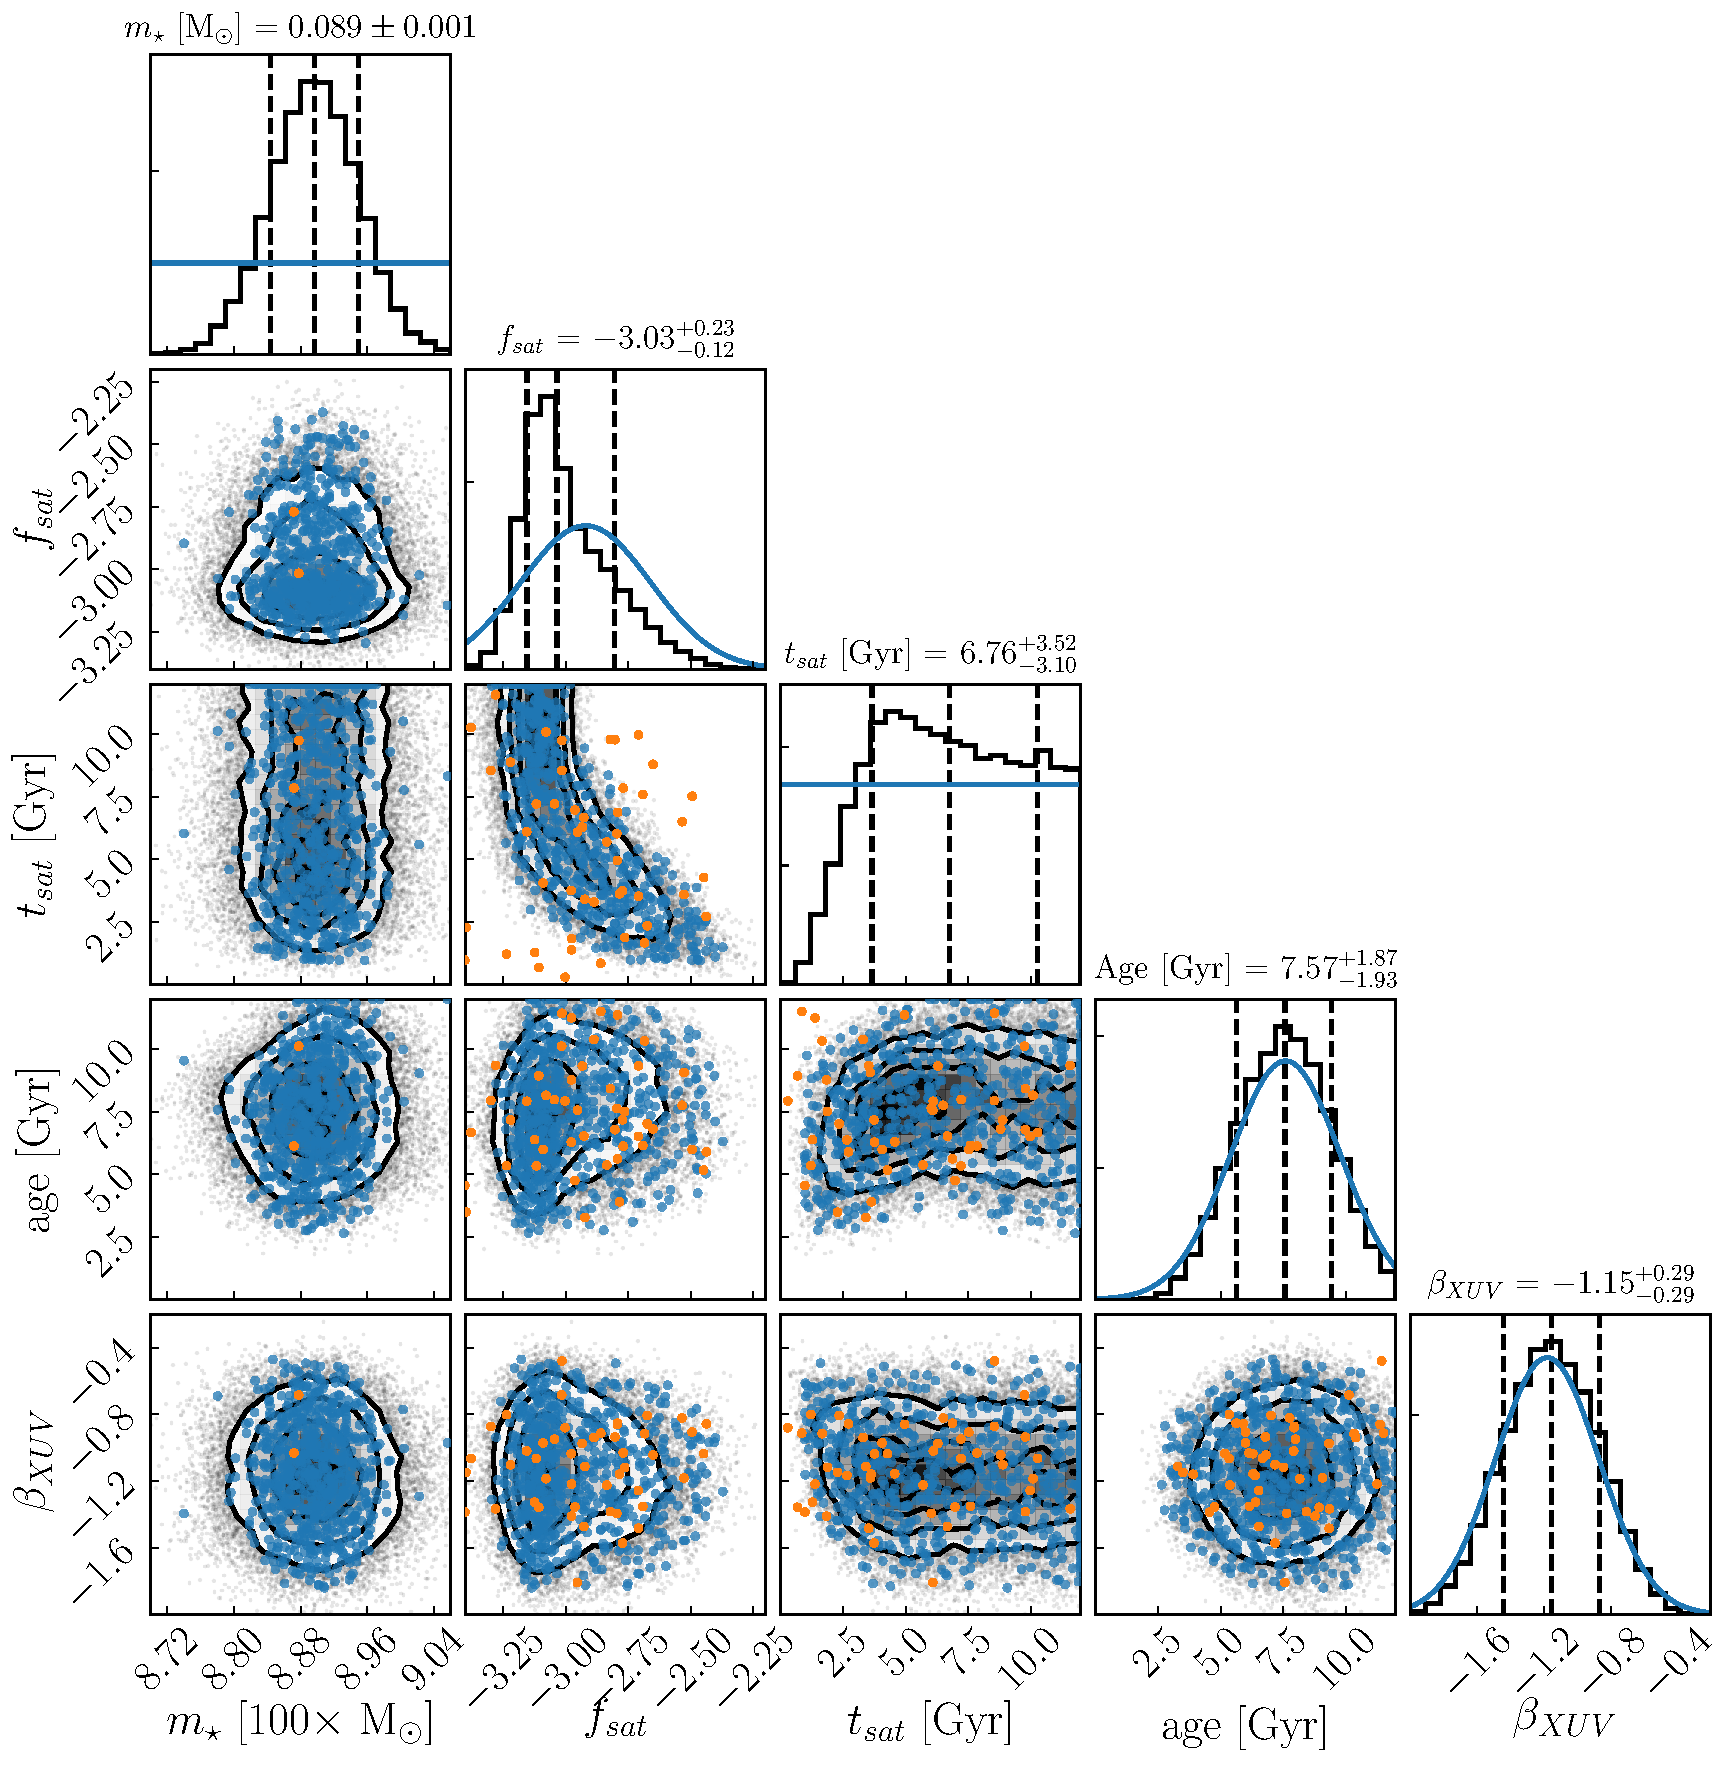
\includegraphics[width=\textwidth]{points.pdf}
   \caption{Same as Fig.~\ref{trap:fig:approx}, but overplotted with the training set for \approxposterior's GP. The orange points display the initial training points whereas the blue points display the points iteratively selected by maximizing the \citet{Kandasamy2017} utility function, Eqn.~(\ref{AP:eq:bape}). By design, \approxposterior selected points to expand its training set in regions of high posterior density improving its GP's predictive accuracy in the most relevant regions of parameter space while seldom wasting computational resources in the low likelihood regions.}%
    \label{AP:fig:points}%
\end{figure}

As demonstrated in \citet{Kandasamy2017}, Eqn.~(\ref{AP:eq:bape}) identifies high-likelihood points where the GP's predictions are uncertain, significantly reducing the cost of training an accurate GP surrogate model. I found that Eqn.~(\ref{AP:eq:agp}) behaves similarly in practice. In Fig.~\ref{AP:fig:points}, I emphasize this behavior by displaying the approximate joint and marginal posterior distribution derived by \approxposterior from \citet{Fleming2020} overplotted with the initial training set in orange and the points selected by sequentially maximizing Eqn.~(\ref{AP:eq:bape}) in blue. See Chapter 6 for additional information on the science underlying this application. Given the small initial training set, \approxposterior successfully selects high-posterior density points in parameter space to augment the GP's training set. Some points are selected in low-likelihood regions early on, typically near the edges of parameter space where the GP's uncertainty was initially large.

\subsection{Convergence} \label{AP:sec:app:convergence}

I assess the convergence of the \approxposterior algorithm by comparing the means of the approximate marginal posterior distributions over successive iterations. I consider an \approxposterior run ``converged" if the differences between the marginal posterior means, relative to the widths of the marginal posteriors, are less than a tolerance parameter, $\epsilon$, for $k_{max}$ consecutive iterations. Effectively, this criterion checks if the expected value of each model parameter over the posterior distribution varies by ${\leq}{\epsilon}$ standard deviations from the previous iteration's expected values. That is, I require the \approxposterior convergence diagnostic $z_{t,j}{\leq}{\epsilon}$ for all $j$, where
\begin{equation}
    z_{t,j} = |\mu_{t,j} - \mu_{t-1,j}| / \sigma_{t-1,j},
\end{equation}
 and $\mu_{t,j}$ and $\sigma_{t,j}$ are the mean and standard deviation of the approximate marginal posterior distribution for the $t^{th}$ iteration and the $j^{th}$ parameter. This quantity is analogous to the ``z-score" commonly used in many statistical tests. Following \citet{Wang2018}, I require this condition to be satisfied for $k_{max}$ consecutive iterations to ensure \approxposterior is producing a consistent result. With this scheme, \approxposterior tolerates deviations from the previous estimate that are less than, or at least consistent with, the previous values given the inherent uncertainty implied by the width of the posterior distribution. For my application explored in Chapter 6, for example, I adopted conservative choices of $\epsilon = 0.1$ and $k_{max} = 5$. 
 
Note that this scheme does not explicitly track the convergence of the width of the marginal distribution for the $j^{th}$ model parameter, e.g. $\sigma_j$, but instead focuses on comparing how the expected value of each model parameter varies over successive \approxposterior iterations. Ensuring that the width of the marginal distribution, and hence the uncertainty in parameter values implied by the data, is critical in any Bayesian inference problem as one of its principle goals is to quantify parameter uncertainties. To address this deficiency, each \approxposterior iteration I visually inspect the estimated joint and marginal posterior distributions to ensure convergence. Since the number of \approxposterior iterations required for convergence is typical of order $n_{\mathrm{max}}=2-3 \times d$ for $d$ model parameters (see $\S$~\ref{AP:app:algo}), it is rather straight-forward to inspect the joint and marginal posterior distributions by eye to assess convergence, i.e. ensuring that the expected values and widths of the marginal posterior distributions approximately converge to similar values over successive iterations. Moreover, analyzing the posterior distributions by eye allows users to assess how the non-linear correlations between model parameters evolve as a function of \approxposterior iteration when assessing convergence and to check if the GP is properly learning the posterior distribution in order to diagnosis any bugs or errors. Therefore the combination of the above convergence scheme and by eye assessment permits users to confidently assess when an \approxposterior run has converged to a suitable tolerance.

In Fig.~\ref{AP:fig:convergence}, I display the convergence diagnostic quantity, $z_t$, as a function of iteration for each model parameter for the \approxposterior run presented in the Chapter 6 for illustrative purposes. In this case, \approxposterior quickly finds a consistent result as $z_t$ decreases below the convergence threshold within the first few iterations. For each parameter, $z_t$ continues to decrease until iteration 3 before stabilizing. The evolution of $z_t$ is not monotonic, however, owing to the stochastic nature of GPs, the hyperparameter optimization scheme, and MCMC sampling that can cause these values to occasionally be slightly worse or better than previous iterations with no real improvement in the posterior accuracy. Requiring convergence over $k_{max}$ consecutive iterations mitigates the impact of this stochasticity.

\begin{figure}
\centering
	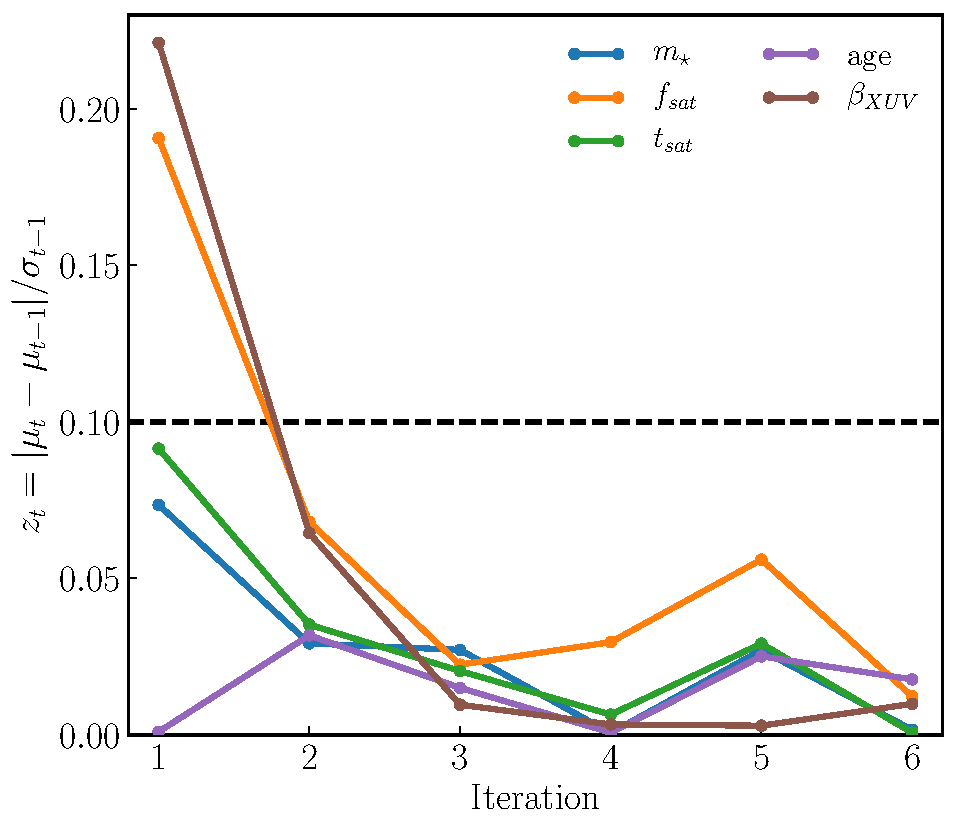
\includegraphics[width=\textwidth]{convergence.pdf}
   \caption{The \approxposterior convergence diagnostic, $z_t$, as a function of iteration for the run presented in the Chapter 6. Note that in \approxposterior, the initial iteration is iteration 0. The black dashed line indicates the adopted convergence threshold of $\epsilon = 0.1$. \approxposterior quickly converges to a consistent and accurate result.}%
    \label{AP:fig:convergence}%
\end{figure}

\subsection{A Simple Example} \label{AP:sec:example}

Here, I demonstrate how to use \approxposterior in practice to reproduce the 2-dimensional (2D) Rosenbrock function inference test examined by \citet{Wang2018}. The 2D Rosenbrock function is a classic optimization test function with a global minimum of 0 at (1,1). The Rosenbrock function exhibits non-linear, banana-like correlations making it a suitable challenge for \approxposterior. \citet{Wang2018} define the 2D Rosenbrock function likelihood as
\begin{equation} \label{AP:eqn:rosenbrock}
l(\textbf{x}) = \exp \left( -\frac{1}{100}(x_1 - 1)^2 - (x_1^2 - x_2)^2 \right)
\end{equation}
where $\textbf{x} = \{ x_1, x_2 \}$. In practice, \approxposterior works with the natural logarithm of Eqn.~(\ref{AP:eqn:rosenbrock}). I follow \citet{Wang2018} and adopt a uniform prior distribution for both $x_1$ and $x_2$ over [-5, 5].

Below, I include a simple Python script for applying \approxposterior to the 2D Rosenbrock inference problem.\footnote{The script is available at \href{https://github.com/dflemin3/approxposterior/blob/master/examples/inference/example.py}{https://github.com/dflemin3/approxposterior/blob/master/examples/inference/example.py}} In the first section, I define algorithm parameters that set the size of the initial training set, $m_0$, and control how \approxposterior operates, i.e. I only run two iterations by setting $n_{max} = 2$. As demonstrated below, this number of iterations is sufficient to reproduce the \citet{Wang2018} result. I also define the hard parameter bounds equal to the prior bounds to prevent the GP from blowing up by trying to learn in forbidden regions of parameter space, e.g. $x_1 > 5$. Next, I create the training set, $T = \{ \theta, y \}$, where the model parameters $\theta = \textbf{x}$ in this case. Note how $y$ is the sum of the lnlikelihood and lnprior distribution, that is, the unnormalized logarithm of the posterior probability in Bayes' Theorem. In \approxposterior notation, the GP iteratively learns $\hat{y} = \hat{f}(\textbf{x})$ as an approximation of $y = f(\textbf{x})$.

As explained above, \approxposterior requires a GP. \approxposterior has a useful convenience function for initializing GPs, \textit{defaultGP}, that creates a GP with a squared exponential kernel and takes care of various bookkeeping tasks for the user behind-the-scenes. In the script, I use this function to initialize the GP and pass it, along with functions that describe the lnlikelihood, lnprior, and how to sample from the prior to the \texttt{ApproxPosterior} object used to perform inference. Finally, I call the \approxposterior \texttt{run} method with the parameters described above and after a few minutes, the inference is complete. Finally, I extract the posterior samples using an \emcee utility function and visualize the joint posterior probability distribution estimated by \approxposterior. I display this distribution in Fig.~\ref{AP:fig:rosenbrock}. 

\inputpython{example.py}{1}{45}

Compare the posterior distribution in Fig.~\ref{AP:fig:rosenbrock} to Figures 1 and 3 from \citet{Wang2018}. The agreement is excellent, validating my implementation in \approxposterior. I also display the points selected by \approxposterior's training set augmentation procedure in red. As expected, the points \approxposterior selected preferentially cluster in regions of high posterior density, improving the accuracy of \approxposterior's GP surrogate model in the relevant regions of parameter space.

\begin{figure}
\centering
	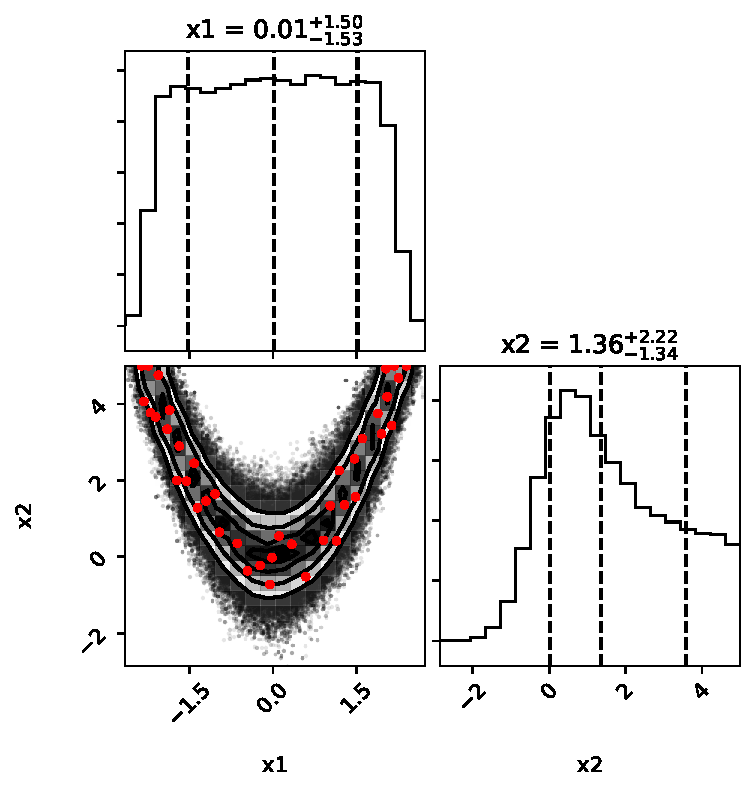
\includegraphics[width=\textwidth]{finalPosterior.pdf}
   \caption{The posterior probability distribution for the 2D Rosenbrock example from \citet{Wang2018} estimated by \approxposterior.  The red points denote points selected by \approxposterior's training set augmentation scheme using the BAPE algorithm. As explained above, \approxposterior preferentially selects points in regions of high posterior density. The posterior distribution estimated by \approxposterior is in good agreement with the results of \citet{Wang2018}, their Figures 1 and 3.}%
    \label{AP:fig:rosenbrock}%
\end{figure}

\subsection{Online Documentation} \label{AP:sec:docs}

I wrote extensive online documentation for \approxposterior that is located on both its main GitHub page\footnote{\href{https://github.com/dflemin3/approxposterior}{https://github.com/dflemin3/approxposterior}} and on an additional public documentation website\footnote{\href{https://dflemin3.github.io/approxposterior/}{https://dflemin3.github.io/approxposterior/}}. The online examples comprise both annotated Jupyter Lab notebooks and commented Python scripts, like the one shown above, to allow new users understand how \approxposterior is called and used in practice. Moreover, the online documentation includes the full \approxposterior API; each parameter in every \approxposterior class and function is fully described, including a definition for each parameter, its data type, and reasonable default values. The online documentation serves to help new users employ \approxposterior in their own research. As the primary author of \approxposterior, I encourage new users to both fully read the online documentation and run all examples before developing scripts for their own application.

\section{Applying \approxposterior to Terrestrial Exoplanet Atmospheric Retrieval} \label{AP:sec:future}

\approxposterior is agnostic to the forward model it learns and is therefore not restricted to working with \vplanet-based lnprobabilities or analytic functions as demonstrated in Chapter 6 and above, respectively. \approxposterior is applicable for a wide array of Bayesian inference problems, particularly those that involve computationally-expensive models as demonstrated in this Chapter and in Chapter 6.  Here, I discuss an additional application of \approxposterior to the inference, or retrieval, of chemical abundances from synthetic transmission spectra of terrestrial exoplanet atmospheres (Lustig-Yaeger et al., in prep).

With future facilities like the James Webb Space Telescope (JWST) eventually coming online, astronomers will likely be able to detect and characterize the first terrestrial exoplanet atmospheres. The most likely targets for this effort are the TRAPPIST-1 planets owing to the system's proximity to Earth, the large relative planetary transit depths, and the small star-planet separations \citep{Gillon2016,Gillon2017,Morley2017,Lustig2019}. Since the TRAPPIST-1 planets all transit, JWST will be able to measure the absorption of stellar light passing though any atmosphere the planets may possess as a function of wavelength, a technique known as transmission spectroscopy. Given suitable theoretical models for an exoplanet's transmission spectra, e.g. \citet{Lincowski2018}, modelers can solve the inference problem of inferring, or retrieving, the abundance of chemical species like O$_2$ in an exoplanet's atmosphere by matching theoretical models of transmission spectra with the observed spectra and uncertainties \citep[e.g.][]{KrissansenTotton2018,Tremblay2020}. Retrievals are another application of Bayesian inference analogous to the case of matching \vplanet outputs with observational constraints discussed in this dissertation.

Retrievals, however, are inherently computationally-expensive tasks because simulating transmission spectra requires not only simulating a physically-plausible exoplanet climate and atmospheric temperature structure \citep{Lincowski2018}, but also requires performing complex radiative transfer simulations \citep[e.g. with SMART, ][]{Meadows1996,Crisp1997}. To mitigate this computational expense, numerous groups have turned to machine learning to bypass this modeling in favor of training a model that maps atmospheric chemical abundances to transmission spectra using neural networks \citep{Waldmann2016,MarquezNeila2018,Zingales2018,Cobb2019,Fisher2019,Himes2020}. In this paradigm, the neural network is trained on a large ($\geq 10^4-10^5$) grid of pre-computed transmission spectra with known atmospheric chemical abundances and planetary properties. The neural network learns an approximate mapping between input planetary physical and atmospheric properties and the transmission spectra, bypassing complex climate and radiative transfer simulations to significantly reduce the computational expense of retrievals.

Although promising, neural network-based approaches suffer two critical limitations. First, neural networks have a large number of parameters and hence require massive grids of pre-computed spectra for training. The size of these grids scales exponentially with the dimensionality of the inference. Simulating this initial grid is of course computationally-expensive. Second, if the theoretical model for the transmission spectra changes, perhaps if new line lists are developed or climate models are refined, the neural network's initial training grid must be recomputed as a previously-trained neural network would have been tuned to out-dated, or at worst, incorrect physics, therefore biasing any retrieved abundances. 

Here, I present work-in-progress from Lustig-Yaeger et al, in prep, to demonstrate that \approxposterior is well-suited to retrievals and provides comparable accuracy as direct inference methods, but requires about 800 times fewer computational resources. I consider the case of inferring the isothermal atmospheric temperature and mixing ratios of H$_2$O and CO$_2$ from a synthetic transmission spectra of TRAPPIST-1e with noise levels comparable to what astronomers expect from JWST \citep{Lincowski2018}. In this case, I consider two retrieval methods (see Lustig-Yaeger et al, in prep. for a complete description). For the first method, I run SMART radiative transfer simulations each $\textbf{x}$ evaluation within an \emcee sampler to derive the posterior distribution. I refer to this method as the ``fiducial" inference method. For the second, I use \approxposterior within \emcee to replace the $\textbf{x}$ evaluation and estimate the posterior distribution. Each method's MCMC chain was run with identical parameters. 

I display the posterior distributions inferred by both methods in Fig.~\ref{AP:fig:comparison}. The fiducial posterior distribution is purple and the \approxposterior-derived distribution is orange. Both the joint and marginal posterior distributions derived by \approxposterior are in excellent with the distributions derived by the fiducial method demonstrating \approxposterior's ability to accurately replace the complex radiative transfer simulations for computing the lnprobability. Note how the marginal constraints, both the best fit value and the uncertainties, derived by both methods listed in Fig.~\ref{AP:fig:comparison} are in good agreement. Since the \approxposterior GP is fundamentally an approximate model for the lnprobability, the agreement between the fiducial and \approxposterior-derived posterior distributions is not perfect as can be seen in Fig.~\ref{AP:fig:comparison}. \approxposterior required about 4,000 SMART simulations total to train its GP whereas \emcee required about 3,000,000 to evaluate the MCMC. In this case, \approxposterior is about ${\sim}800$ times more efficient than the fiducial method, a dramatic reduction in computational cost without appreciably reducing the accuracy on the inference. Clearly, \approxposterior offers a promising method to enable rapid and accurate Bayesian inference for computationally-expensive models.

\begin{figure}
\centering
	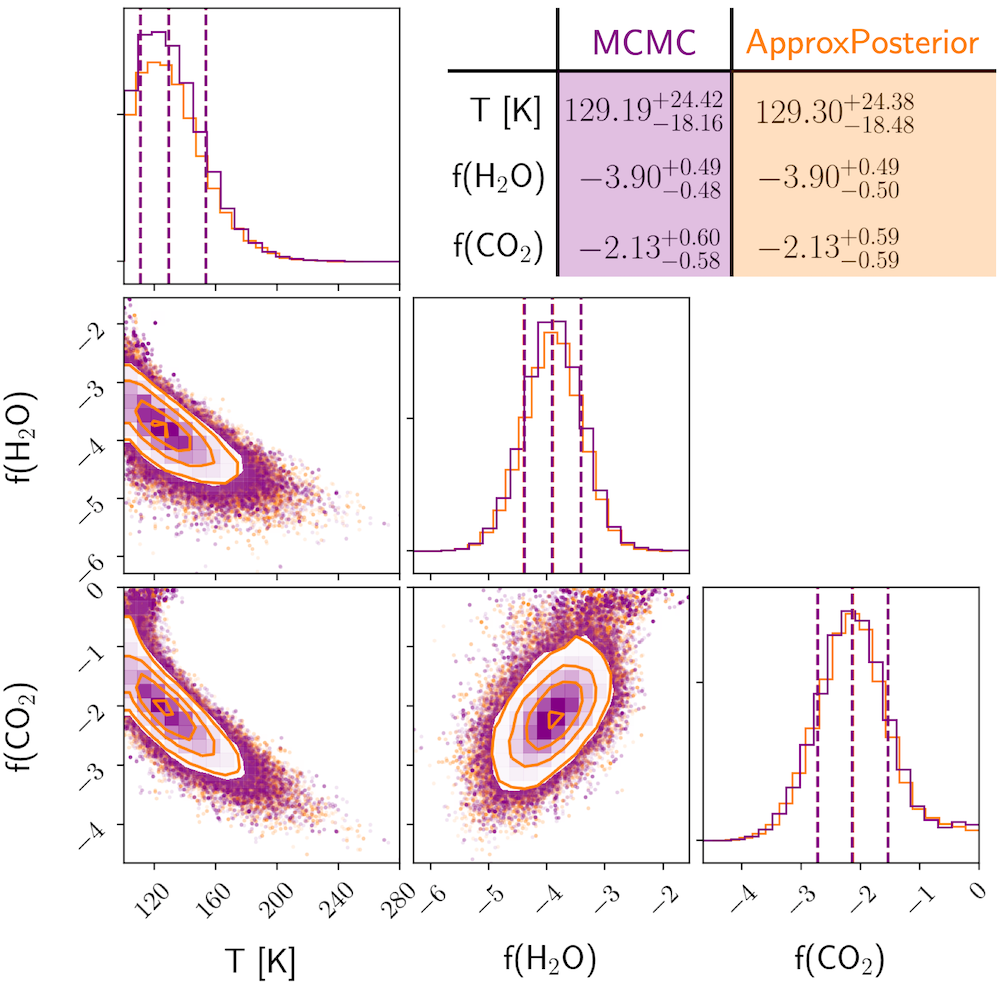
\includegraphics[width=\textwidth]{emceeAPComparison.png}
   \caption{Joint and marginal posterior probability distributions derived by \emcee (purple) and \approxposterior (orange) from an atmospheric retrieval of a simulated noised JWST transmission spectrum of TRAPPIST-1e (used with permission from Lustig-Yaeger et al., in prep). This retrieval experiment attempts to infer the isothermal atmospheric temperature, $T$, and the mixing ratios of H$_2$O and CO$_2$. \approxposterior accurately recovers both the nontrivial correlations between model parameters and marginal parameter constraints as did \emcee, within Monte Carlo error, but requiring about 800 times fewer computational resources.}%
    \label{AP:fig:comparison}%
\end{figure}

\section{Conclusions}

In this Chapter, I introduced \approxposterior, an open-source Python machine learning package that uses GP regression for rapid and accurate approximate Bayesian inference. I outlined the mathematics and algorithm underpinning \approxposterior and examined its practical application. After explaining the \approxposterior algorithm and convergence scheme, I sketched an in-progress research project using \approxposterior and demonstrated that it was as accurate as direct inference methods using \emcee, but required 800 times fewer computational resources. 



\printendnotes

%
% ==========   Bibliography
%
%\nocite{*}   % include everything in the uwthesis.bib file
\bibliographystyle{apalike} % plain if not natbib
\bibliography{thesisBib}
%
% ==========   Appendices
%

\appendix
\raggedbottom\sloppy

\chapter{Vita}
I am David P. Fleming. When I want to procrastinate on the much more important sections of my thesis, I will complete my vita.


\end{document}
